% =====================================================================
%  ROTEIRO DE AULA PRÁTICA (60 MIN)
%  Plataforma Didática RISC-V com Aceleração Neural em FPGA
%  Instituto Mauá de Tecnologia - Engenharia de Computação
%  Disciplina: Arquitetura e Organização de Computadores
% ---------------------------------------------------------------------
%  COMPILAÇÃO
%    Recomendado: XeLaTeX ou LuaLaTeX (usa a fonte Open Sans, se instalada)
%        latexmk -xelatex roteiro_experimentos.tex
%    Também funciona com pdfLaTeX (usa o pacote opensans, se disponível):
%        latexmk -pdf roteiro_experimentos.tex
%    Rode duas vezes (a capa usa coordenadas "remember picture").
%
%  CHAVES DE CONFIGURAÇÃO (logo abaixo)
%    \modoimpressaotrue  -> fundo branco (economiza tinta ao imprimir)
%    \modoimpressaofalse -> tema escuro, igual à apresentação do TCC
%    \gabaritotrue       -> versão do PROFESSOR (respostas esperadas visíveis)
%    \gabaritofalse      -> versão do ALUNO
% =====================================================================
\documentclass[11pt,a4paper]{article}

% ------------------------- CHAVES ------------------------------------
\newif\ifmodoimpressao
\newif\ifgabarito
\modoimpressaofalse   % <- troque para \modoimpressaotrue para imprimir
\gabaritofalse        % <- troque para \gabaritotrue para a versão do professor

% ------------------------- MOTOR / FONTES ----------------------------
\usepackage{iftex}
\ifPDFTeX
  \usepackage[T1]{fontenc}
  \usepackage[utf8]{inputenc}
  \IfFileExists{opensans.sty}
    {\usepackage[default,scale=0.95]{opensans}}
    {\usepackage[scaled]{helvet}\renewcommand\familydefault{\sfdefault}}
  \IfFileExists{zi4.sty}{\usepackage[scaled=0.88]{zi4}}{}
\else
  \usepackage{fontspec}
  \IfFontExistsTF{Open Sans}
    {\setmainfont{Open Sans}[Scale=0.95]}
    {\IfFontExistsTF{TeX Gyre Heros}{\setmainfont{TeX Gyre Heros}}{}}
  \IfFontExistsTF{DejaVu Sans Mono}
    {\setmonofont{DejaVu Sans Mono}[Scale=0.82]}{}
\fi
% letras e dígitos da matemática na mesma fonte do texto (opcional)
\IfFileExists{mathastext.sty}{\usepackage[italic]{mathastext}}{}

\IfFileExists{brazil.ldf}
  {\usepackage[brazil]{babel}}
  {\usepackage[provide=*,brazilian]{babel}}

% ------------------------- PACOTES -----------------------------------
\usepackage[a4paper,left=2.1cm,right=2.1cm,top=2.6cm,bottom=2.3cm,
            headsep=0.9cm,footskip=1.1cm]{geometry}
\usepackage{amsmath,amssymb}
\usepackage[table]{xcolor}
\usepackage{tikz}
\usetikzlibrary{calc,positioning,arrows.meta}
\usepackage{listings}
\usepackage[most]{tcolorbox}
\usepackage{eso-pic}
\usepackage{fancyhdr}
\usepackage{enumitem}
\usepackage{needspace}
\usepackage{tabularx,array}
\renewcommand{\tabularxcolumn}[1]{m{#1}}
\usepackage{microtype}
\usepackage[hidelinks]{hyperref}

% ------------------------- PALETA ------------------------------------
% Cores extraídas da identidade visual da apresentação do TCC.
\ifmodoimpressao
  \definecolor{fundo}{HTML}{FFFFFF}
  \definecolor{painel}{HTML}{F4F6F9}
  \definecolor{painelB}{HTML}{E9EDF2}
  \definecolor{borda}{HTML}{C9D0DA}
  \definecolor{texto}{HTML}{1E222A}
  \definecolor{suave}{HTML}{5B6471}
  \definecolor{titulo}{HTML}{0B0D12}
  \definecolor{laranja}{HTML}{E07B00}
  \definecolor{azul}{HTML}{1F6FD1}
  \definecolor{verde}{HTML}{2E9A55}
  \definecolor{vermelho}{HTML}{C81E25}
  \definecolor{roxo}{HTML}{7A2BE0}
  \definecolor{ambar}{HTML}{B88000}
  \definecolor{magenta}{HTML}{A51FC7}
  \definecolor{codigoinline}{HTML}{1F5FAF}
  \definecolor{linhacirc}{HTML}{9AA3AF}
\else
  \definecolor{fundo}{HTML}{0B0D12}
  \definecolor{painel}{HTML}{141821}
  \definecolor{painelB}{HTML}{1C212C}
  \definecolor{borda}{HTML}{2E3542}
  \definecolor{texto}{HTML}{E6E8EB}
  \definecolor{suave}{HTML}{9AA3AF}
  \definecolor{titulo}{HTML}{FFFFFF}
  \definecolor{laranja}{HTML}{F7931E}
  \definecolor{azul}{HTML}{4A9BF5}
  \definecolor{verde}{HTML}{4DB870}
  \definecolor{vermelho}{HTML}{E0262E}
  \definecolor{roxo}{HTML}{8E3CF7}
  \definecolor{ambar}{HTML}{F2B530}
  \definecolor{magenta}{HTML}{D63AF9}
  \definecolor{codigoinline}{HTML}{8CC4FF}
  \definecolor{linhacirc}{HTML}{FFFFFF}
\fi
\colorlet{gab}{verde}
\colorlet{acc}{laranja}   % cor de destaque do experimento corrente

\pagecolor{fundo}
\setlength{\parindent}{0pt}
\AtBeginDocument{\color{texto}}

% ------------------------- DECORAÇÃO DAS PÁGINAS ----------------------
% Trilhas de circuito nos cantos (como nos slides). Não aparecem na capa.
\newcommand{\anel}[2]{\draw[#1,line width=0.8pt,fill=fundo] #2 circle (0.075);}
\newcommand{\losango}[2]{\fill[#1,rotate around={45:#2}] #2 ++(-0.1,-0.1) rectangle ++(0.2,0.2);}
\newcommand{\losangovazado}[2]{\draw[#1,line width=0.9pt,rotate around={45:#2}] #2 ++(-0.1,-0.1) rectangle ++(0.2,0.2);}
\AddToShipoutPictureBG{%
  \ifnum\value{page}>1
  \AtPageLowerLeft{%
    \begin{tikzpicture}[x=1cm,y=1cm]
      \useasboundingbox (0,0) rectangle (21,29.7);
      \begin{scope}[linhacirc,line width=0.7pt]
        \draw (21.3,29.2) -- (20.5,28.4) -- (19.5,28.4) -- (19.0,27.9);
        \draw (21.3,28.5) -- (20.8,28.0) -- (20.8,27.7);
        \anel{linhacirc}{(19.0,27.9)}
        \anel{laranja}{(20.8,27.62)}
        \draw (21.3,1.95) -- (20.6,1.25) -- (19.45,1.25);
        \draw (21.3,1.25) -- (20.8,0.75) -- (19.75,0.75);
        \draw (21.3,0.55) -- (21.0,0.25) -- (20.3,0.25);
        \anel{verde}{(19.37,1.25)}
        \anel{linhacirc}{(19.67,0.75)}
        \anel{laranja}{(20.22,0.25)}
      \end{scope}
      \losangovazado{laranja}{(19.9,29.25)}
      \losango{verde}{(18.3,28.75)}
      \losangovazado{roxo}{(20.35,29.0)}
      \losango{vermelho}{(20.1,28.05)}
      \losango{roxo}{(20.35,1.65)}
      \losango{verde}{(20.05,0.6)}
    \end{tikzpicture}}%
  \fi}

% ------------------------- CABEÇALHO / RODAPÉ -------------------------
\pagestyle{fancy}
\fancyhf{}
\renewcommand{\headrulewidth}{0pt}
\fancyhead[L]{\footnotesize\color{suave}\textbf{\color{laranja}PLATAFORMA DIDÁTICA RISC-V}\enspace\textperiodcentered\enspace Roteiro de Aula Prática%
  \ifgabarito\enspace\textperiodcentered\enspace\textbf{\color{gab}VERSÃO DO PROFESSOR}\fi}
\fancyfoot[L]{\footnotesize\color{suave}Instituto Mauá de Tecnologia\enspace\textperiodcentered\enspace Engenharia de Computação}
\fancyfoot[R]{\footnotesize\color{suave}\tikz[baseline=-0.1ex]{\foreach \i in {0,1,2}{\fill[laranja] (\i*0.1,-0.02) rectangle ++(0.06,0.28);}}\hspace{0.4em}\textbf{\color{titulo}\thepage}\hspace{2.2cm}}

% ------------------------- ÍCONES (TikZ) ------------------------------
\newcommand{\icChip}[1][acc]{\tikz[baseline=-0.3em,x=1em,y=1em]{%
  \draw[#1,line width=0.8pt,rounded corners=0.6pt] (-0.3,-0.3) rectangle (0.3,0.3);
  \draw[#1,line width=0.6pt] (-0.12,-0.12) rectangle (0.12,0.12);
  \foreach \p in {-0.15,0,0.15}{\draw[#1,line width=0.55pt] (\p,0.3)--(\p,0.45) (\p,-0.3)--(\p,-0.45) (0.3,\p)--(0.45,\p) (-0.3,\p)--(-0.45,\p);}}}
\newcommand{\icRelogio}[1][acc]{\tikz[baseline=-0.3em,x=1em,y=1em]{%
  \draw[#1,line width=0.8pt] (0,0) circle (0.36); \draw[#1,line width=0.8pt,line cap=round] (0,0.2)--(0,0)--(0.15,-0.08);}}
\newcommand{\icCheck}[1][azul]{\tikz[baseline=-0.3em,x=1em,y=1em]{%
  \fill[#1] (0,0) circle (0.42); \draw[white,line width=1.3pt,line cap=round,line join=round] (-0.2,0.0)--(-0.05,-0.15)--(0.22,0.15);}}
\newcommand{\icOlho}[1][acc]{\tikz[baseline=-0.3em,x=1em,y=1em]{%
  \draw[#1,line width=0.8pt] (-0.42,0) .. controls (-0.15,0.32) and (0.15,0.32) .. (0.42,0) .. controls (0.15,-0.32) and (-0.15,-0.32) .. (-0.42,0); \fill[#1] (0,0) circle (0.12);}}
\newcommand{\icLampada}[1][acc]{\tikz[baseline=-0.3em,x=1em,y=1em]{%
  \draw[#1,line width=0.8pt] (-0.12,-0.12) arc[start angle=235,end angle=-55,radius=0.3]; \draw[#1,line width=0.8pt] (-0.12,-0.12)--(-0.12,-0.28)--(0.12,-0.28)--(0.12,-0.12); \draw[#1,line width=0.8pt] (-0.1,-0.4)--(0.1,-0.4);}}
\newcommand{\icAntena}[1][acc]{\tikz[baseline=-0.3em,x=1em,y=1em]{%
  \fill[#1] (0,-0.15) circle (0.08); \draw[#1,line width=0.8pt] (-0.22,0.03) arc[start angle=135,end angle=45,radius=0.31]; \draw[#1,line width=0.8pt] (-0.38,0.19) arc[start angle=135,end angle=45,radius=0.54]; \draw[#1,line width=0.8pt] (0,-0.15)--(0,-0.45);}}
\newcommand{\icPrancheta}[1][acc]{\tikz[baseline=-0.3em,x=1em,y=1em]{%
  \draw[#1,line width=0.8pt,rounded corners=0.8pt] (-0.3,-0.42) rectangle (0.3,0.36); \fill[#1] (-0.13,0.3) rectangle (0.13,0.45);
  \foreach \y in {0.12,-0.05,-0.22}{\draw[#1,line width=0.6pt] (-0.17,\y)--(0.17,\y);}}}
\newcommand{\icAlerta}[1][acc]{\tikz[baseline=-0.3em,x=1em,y=1em]{%
  \draw[#1,line width=0.8pt,line join=round] (0,0.38)--(0.42,-0.36)--(-0.42,-0.36)--cycle; \draw[#1,line width=0.9pt] (0,0.14)--(0,-0.1); \fill[#1] (0,-0.22) circle (0.04);}}

% ------------------------- ELEMENTOS DE TEXTO -------------------------
\newcommand{\barras}[2][0.62]{\tikz[baseline=0pt]{\foreach \i in {0,1,2}{\fill[#2] (\i*#1*0.36,0) rectangle ++(#1*0.22,#1);}}}
\newcommand{\gui}[1]{\textbf{\color{titulo}#1}}                 % nome de painel/área da GUI
\newcommand{\cod}[1]{\texttt{\color{codigoinline}#1}}           % código inline
\newtcbox{\btn}{on line, colback=painelB, colframe=acc, boxrule=0.5pt,
  arc=2.5pt, boxsep=0pt, left=3pt, right=3pt, top=1.6pt, bottom=1.2pt,
  fontupper=\ttfamily\footnotesize\color{titulo}}                % botão da GUI
\newcommand{\numcirc}[1]{\tikz[baseline=(n.base)]\node[circle,draw=acc,line width=0.8pt,
  inner sep=0pt,minimum size=1.3em,font=\scriptsize\bfseries,text=titulo](n){#1};}
\newtcbox{\chip}{on line, colback=fundo, colframe=acc, boxrule=0.6pt, arc=7pt,
  boxsep=0pt, left=6pt, right=7pt, top=2.2pt, bottom=2.2pt, fontupper=\footnotesize\color{texto}}

\tcbset{colupper=texto, collower=texto, coltitle=titulo, colback=painel, colframe=borda}

\newcommand{\titulopagina}[2]{%
  \colorlet{acc}{#1}%
  {\noindent\barras[0.72]{acc}\hspace{0.35cm}{\fontsize{25}{30}\selectfont\bfseries\color{titulo}#2}\par}\vspace{4mm}}
\newcommand{\secao}[1]{\par\needspace{5\baselineskip}\vspace{4mm}%
  \noindent\barras[0.36]{acc}\hspace{0.18cm}{\bfseries\color{titulo}\MakeUppercase{#1}}\par\vspace{2mm}}
\newcommand{\rotulo}[2][acc]{{\footnotesize\bfseries\color{#1}#2}}

% listas
\newlist{passos}{enumerate}{1}
\setlist[passos]{label=\protect\numcirc{\arabic*}, leftmargin=2.0em, labelsep=0.45em,
  itemsep=2pt, topsep=2pt, parsep=0pt}
\setlist[itemize]{label={\color{acc}\small$\blacktriangleright$}, leftmargin=1.4em, itemsep=2pt, parsep=0pt, topsep=2pt}

% ------------------------- CAIXAS -------------------------------------
\newtcolorbox{conceito}{enhanced, colback=painel, frame hidden, halign=left,
  borderline west={3pt}{0pt}{acc}, arc=3pt, left=9pt, right=8pt, top=5pt, bottom=5pt,
  fontupper=\small, before upper={\rotulo{\icLampada\ CONCEITO}\par\smallskip}}

\newtcolorbox{observe}{enhanced, breakable, colback=fundo, frame hidden, before upper app={}, halign=left,
  borderline={0.7pt}{0pt}{acc, dash pattern=on 3pt off 2pt}, arc=4pt,
  left=7pt, right=7pt, top=5pt, bottom=5pt, fontupper=\small,
  before upper={\rotulo{\icOlho\ OBSERVE E DISCUTA EM GRUPO}\par\smallskip}}

\newtcolorbox{tarefabox}[1]{enhanced, breakable, colback=fundo, colframe=vermelho, boxrule=1.2pt,
  arc=7pt, left=11pt, right=11pt, top=12pt, bottom=10pt, fontupper=\small,
  attach boxed title to top left={xshift=12pt,yshift=-9pt},
  boxed title style={colback=vermelho, colframe=vermelho, arc=4pt, boxrule=0pt, left=6pt, right=6pt, top=2pt, bottom=2pt},
  coltitle=white, fonttitle=\footnotesize\bfseries,
  title={\icPrancheta[white]\ #1}}

\newtcolorbox{gabbox}{colback=gab!12!fundo, colframe=gab, colupper=texto, boxrule=0pt, leftrule=2.5pt,
  sharp corners, left=8pt, right=6pt, top=3pt, bottom=3pt, fontupper=\small,
  before upper={{\bfseries\color{gab}Gabarito:}\ }}

\newtcolorbox{nota}[1][azul]{enhanced, colback=painel, colframe=#1, boxrule=0.8pt, arc=6pt,
  left=9pt, right=9pt, top=6pt, bottom=6pt, fontupper=\small}

% ------------------------- GABARITO -----------------------------------
% \esperado{...}: resposta esperada de uma pergunta (só na versão do professor)
\newcommand{\esperado}[1]{\ifgabarito\par\vspace{0.5mm}{\footnotesize\color{gab}\textbf{Esperado:} #1}\fi}

% ------------------------- CÓDIGO -------------------------------------
\ifmodoimpressao\definecolor{codigofundo}{HTML}{F4F6F9}\else\definecolor{codigofundo}{HTML}{07090D}\fi
\lstdefinelanguage{riscv}{
  alsoletter={._},
  morekeywords={li,beq,bne,sw,lw,add,addi,mv,j,wfi},
  morekeywords=[2]{.global,_start,fib_loop,end},
  sensitive=true, morecomment=[l]{\#}}
\lstset{
  basicstyle=\ttfamily\scriptsize\color{texto},
  keywordstyle=\color{azul}\bfseries,
  keywordstyle=[2]\color{ambar},
  commentstyle=\color{suave}\itshape,
  emphstyle=\color{laranja},
  columns=fullflexible, keepspaces=true, showstringspaces=false,
  aboveskip=0pt, belowskip=0pt, tabsize=4}
\newtcblisting{codigo}[1][]{enhanced, listing only, colback=codigofundo, colframe=borda,
  boxrule=0.5pt, arc=4pt, left=4pt, right=4pt, top=3pt, bottom=3pt, listing options={#1}}

% ------------------------- EXPERIMENTO ------------------------------------
\newcounter{experimento}
% \estacao{cor}{número}{título}{aba da GUI}{execução}{tempo}
\newcommand{\estacao}[6]{%
  \clearpage
  \colorlet{acc}{#1}%
  \setcounter{experimento}{\numexpr#2\relax}%
  \noindent{\fontsize{30}{30}\selectfont\bfseries\color{acc}#2}\hspace{3mm}%
  \begin{minipage}[b]{0.83\linewidth}
    {\large\bfseries\color{titulo}#3}\par\vspace{1.2mm}
    \chip{\icChip\ \textbf{Aba:} #4}\hspace{1mm}\chip{\icAlerta\ \textbf{Execução:} #5}
  \end{minipage}\par
  \vspace{1.5mm}{\color{borda}\hrule height 0.6pt}\vspace{3mm}}
% linha de trade-off dentro do conceito
\newcommand{\tradeoff}[1]{\par\vspace{1.5mm}{\rotulo{TRADE-OFF:}\ #1}}
% bloco de passos
\newlength{\espacobloco}\setlength{\espacobloco}{3mm}
\newenvironment{faca}{\par\vspace{\espacobloco}\raggedright\rotulo{\icChip\ FAÇA}\par\small}{\par}
% perguntas ao final do experimento (numeradas 1.1, 1.2, ...)
% Na versão do professor, as perguntas e respostas esperadas ficam em uma página própria.
\newlist{perguntas}{enumerate}{1}
\setlist[perguntas]{label={\bfseries\color{acc}\theexperimento.\arabic*}, leftmargin=2.2em, labelsep=0.5em,
  itemsep=\ifgabarito 6pt\else 4pt\fi, topsep=2pt, parsep=0pt}
\newenvironment{discuta}{\par\ifgabarito\clearpage\else\vspace{\espacobloco}\fi\begin{observe}\begin{perguntas}}{\end{perguntas}\end{observe}}
\newcommand{\borda}[1]{\par\vspace{\espacobloco}{\small\icAntena[titulo]\ \rotulo[titulo]{NA BORDA:}\ #1}\par}

% =====================================================================
\begin{document}

% ============================== CAPA =================================
\thispagestyle{empty}

\begin{tikzpicture}[remember picture, overlay, x=1cm, y=1cm]
  \coordinate (O) at (current page.south west);
  \begin{scope}[shift={(O)}]
    % ----- chip com trilhas (inspirado na capa da apresentação) -----
    \begin{scope}[shift={(14.4,9.0)}, rotate=45]
      \def\pa{2.25}   % meio lado da moldura
      \def\pp{2.95}   % ponta dos pinos
      \begin{scope}[linhacirc, line width=0.8pt]
        % face NE: segue na direção da face e dobra para cima
        \foreach \t/\l/\m/\c in {-1.5/1.6/1.8/linhacirc, -0.5/1.0/2.9/laranja, 0.5/0.4/2.0/linhacirc}{
          \draw (\pp,\t) -- ++(0:\l) -- ++(45:\m);
          \anel{\c}{($(\pp,\t)+(0:\l)+(45:\m)$)}}
        % face NO: trilhas retas na diagonal
        \foreach \t/\l/\c in {-0.5/2.6/linhacirc, 0.5/1.5/verde, 1.5/2.1/linhacirc}{
          \draw (\t,\pp) -- ++(90:\l);
          \anel{\c}{($(\t,\pp)+(90:\l)$)}}
        % face SO: segue na direção da face e dobra para baixo
        \foreach \t/\l/\m/\c in {-0.5/0.5/2.2/linhacirc, 0.5/1.1/1.4/verde, 1.5/1.7/2.4/linhacirc}{
          \draw (-\pp,\t) -- ++(180:\l) -- ++(225:\m);
          \anel{\c}{($(-\pp,\t)+(180:\l)+(225:\m)$)}}
        % face SE: trilhas retas na diagonal
        \foreach \t/\l/\c in {-1.5/1.4/linhacirc, -0.5/2.4/laranja, 0.5/1.7/linhacirc}{
          \draw (\t,-\pp) -- ++(270:\l);
          \anel{\c}{($(\t,-\pp)+(270:\l)$)}}
      \end{scope}
      % pinos
      \foreach \t in {-1.5,-0.5,0.5,1.5}{
        \fill[vermelho] (\t-0.19,\pa-0.2) rectangle (\t+0.19,\pp);
        \fill[vermelho] (\t-0.19,-\pa+0.2) rectangle (\t+0.19,-\pp);
        \fill[vermelho] (\pa-0.2,\t-0.19) rectangle (\pp,\t+0.19);
        \fill[vermelho] (-\pa+0.2,\t-0.19) rectangle (-\pp,\t+0.19);
      }
      \fill[fundo] (-\pa+0.08,-\pa+0.08) rectangle (\pa-0.08,\pa-0.08);
      \draw[laranja, line width=1.4pt, rounded corners=2pt] (-\pa,-\pa) rectangle (\pa,\pa);
      % núcleo com bordas dentadas
      \fill[laranja] (-1.55,-1.55) rectangle (1.55,1.55);
      \foreach \t in {-1.05,-0.35,0.35,1.05}{
        \fill[fundo] (\t-0.1,1.42) rectangle (\t+0.1,1.56);
        \fill[fundo] (\t-0.1,-1.42) rectangle (\t+0.1,-1.56);
        \fill[fundo] (1.42,\t-0.1) rectangle (1.56,\t+0.1);
        \fill[fundo] (-1.42,\t-0.1) rectangle (-1.56,\t+0.1);
      }
    \end{scope}
    % losangos soltos
    \losango{verde}{(18.9,26.4)}
    \losangovazado{laranja}{(19.6,25.5)}
    \losango{azul}{(18.4,24.7)}
    \losango{laranja}{(19.3,11.6)}
    \losango{laranja}{(19.65,11.25)}
    \losango{vermelho}{(9.6,13.0)}
    \losango{verde}{(18.6,3.6)}
    \losangovazado{verde}{(11.2,4.2)}

    % ----- títulos -----
    \node[anchor=north west, inner sep=0] at (2.0,27.0) {%
      \tcbox[on line, colback=fundo, colframe=laranja, boxrule=0.8pt, arc=8pt, boxsep=0pt,
        left=8pt, right=8pt, top=3pt, bottom=3pt]{\footnotesize\bfseries\color{laranja}ROTEIRO DE AULA PRÁTICA \textperiodcentered\ 60 MINUTOS}};
    \ifgabarito
      \node[anchor=north west, inner sep=0] at (9.35,27.0) {%
        \tcbox[on line, colback=gab, colframe=gab, arc=8pt, boxsep=0pt, left=8pt, right=8pt, top=3pt, bottom=3pt]{\footnotesize\bfseries\color{white}VERSÃO DO PROFESSOR}};
    \fi
    \node[anchor=north west, inner sep=0, text=titulo, font=\bfseries\fontsize{30}{34}\selectfont] at (1.95,25.1) {PLATAFORMA DIDÁTICA};
    \node[anchor=north west, inner sep=0, text=laranja, font=\bfseries\fontsize{96}{100}\selectfont] at (1.65,23.7) {RISC-V};
    \node[anchor=north west, inner sep=0, text=azul, font=\bfseries\fontsize{28}{34}\selectfont, align=left] at (1.95,20.35) {COM ACELERAÇÃO\\NEURAL EM FPGA};
    \draw[vermelho, line width=1.2pt] (2.0,17.3) -- (4.2,17.3);
    \draw[laranja, line width=1.2pt] (4.2,17.3) -- (6.4,17.3);
    \node[anchor=north west, inner sep=0, text width=12cm, align=left] at (2.0,16.85) {%
      {\large\bfseries\color{titulo}Arquitetura e Organização de Computadores}\\[1.5mm]
      {\small\color{suave}7 experimentos, do núcleo multiciclo à inteligência artificial na borda}};

    % ----- instituição -----
    \IfFileExists{./assets/logo.png}
      {\node[anchor=south west, inner sep=0] at (2.0,3.5) {\includegraphics[height=1.3cm]{./assets/logo.png}};}
      {\node[anchor=south west, inner sep=0, align=left] at (2.0,3.5) {{\bfseries\color{titulo}Instituto Mauá de Tecnologia}\\{\bfseries\color{titulo}Engenharia de Computação}};}
    \node[anchor=south west, inner sep=0, align=left, font=\scriptsize, text=suave] at (2.0,1.3) {%
      \textbf{Autores:} André Maiolini, Durval Soranz, Leonardo Amadio,\\Lucas Castanho e Estevan Feher\\[0.6mm]
      \textbf{Orientadores:} Prof.\ Me.\ Nuncio Perrella e\\Prof.\ Dr.\ Angelo Sebastião Zanini};
  \end{scope}
\end{tikzpicture}
\clearpage

% ============================ PLANO DA AULA ============================
\titulopagina{azul}{PLANO DA AULA}

\vspace{5mm}

Em 60 minutos, cada grupo percorre \textbf{sete experimentos} com sua própria FPGA, uma por aba da interface gráfica. Cada experimento
liga um conceito clássico da disciplina a um módulo do SoC RISC-V que está por trás de sistemas modernos de
\textbf{computação na borda}. A aula termina com a entrega, em grupo, das respostas às perguntas de cada experimento.

\vspace{3mm}
\begin{center}
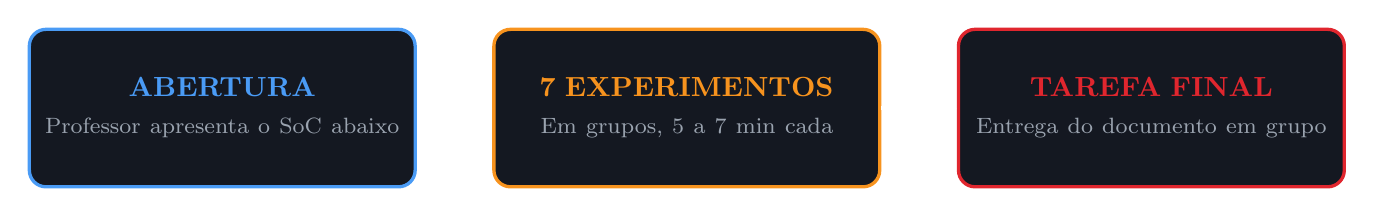
\begin{tikzpicture}[x=1cm,y=1cm,
    etapa/.style={draw=#1, line width=1.2pt, rounded corners=6pt, fill=painel,
      minimum width=4.9cm, minimum height=2.0cm, text width=4.5cm, align=center, inner sep=3pt},
    seta/.style={-{Triangle[length=2.4mm,width=2.4mm]}, line width=1.4pt, titulo}]
  \node[etapa=azul] (a) at (0,0) {{\bfseries\color{azul}ABERTURA}\\[0.5mm]{\footnotesize\color{suave}Professor apresenta o SoC abaixo}};
  \node[etapa=laranja] (b) at (5.9,0) {{\bfseries\color{laranja}7 EXPERIMENTOS}\\[0.5mm]{\footnotesize\color{suave}Em grupos, 5 a 7 min cada}};
  \node[etapa=vermelho] (c) at (11.8,0) {{\bfseries\color{vermelho}TAREFA FINAL}\\[0.5mm]{\footnotesize\color{suave}Entrega do documento em grupo}};
  \draw[seta] (a.east) -- (b.west);
  \draw[seta] (b.east) -- (c.west);
\end{tikzpicture}
\end{center}
\vspace{5mm}

\secao{Abertura: o SoC da plataforma}
\vspace{5mm}
\begin{center}
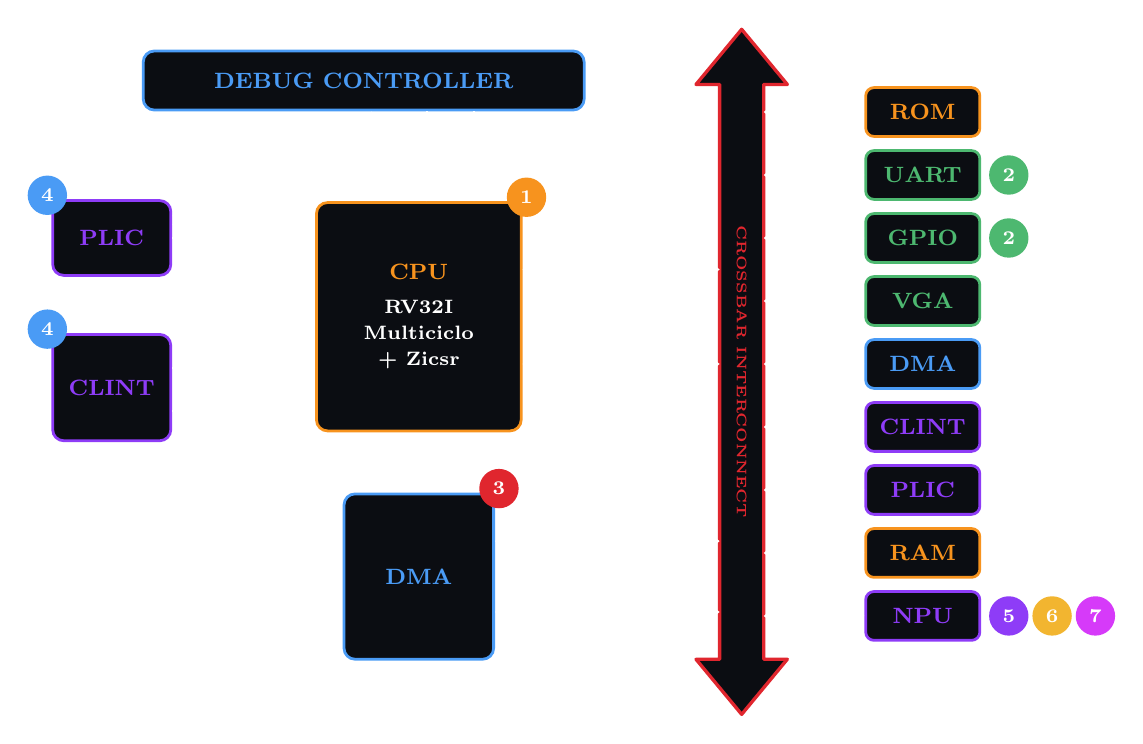
\begin{tikzpicture}[x=1cm,y=1cm, font=\footnotesize\bfseries,
    blk/.style={draw=#1, line width=1pt, rounded corners=4pt, fill=fundo, text=#1, align=center},
    per/.style={draw=#1, line width=1pt, rounded corners=3pt, fill=fundo, text=#1, minimum width=1.45cm, minimum height=0.62cm},
    bus/.style={{Triangle[length=1.6mm,width=2.6mm]}-{Triangle[length=1.6mm,width=2.6mm]}, line width=0.9pt, titulo},
    sig/.style={-{Triangle[length=1.4mm,width=1.6mm]}, line width=0.7pt, titulo},
    badge/.style={circle, fill=#1, text=white, inner sep=0pt, minimum size=0.5cm, font=\scriptsize\bfseries}]
  \node[blk=azul, minimum width=5.6cm, minimum height=0.75cm] (dbg) at (3.2,6.9) {DEBUG CONTROLLER};
  \node[blk=laranja, minimum width=2.6cm, minimum height=2.9cm] (cpu) at (3.9,3.9) {CPU\\[1mm]{\color{titulo}\scriptsize RV32I}\\{\color{titulo}\scriptsize Multiciclo}\\{\color{titulo}\scriptsize + Zicsr}};
  \node[blk=roxo, minimum width=1.5cm, minimum height=0.95cm] (plic) at (0.0,4.9) {PLIC};
  \node[blk=roxo, minimum width=1.5cm, minimum height=1.35cm] (clint) at (0.0,3.0) {CLINT};
  \node[blk=azul, minimum width=1.9cm, minimum height=2.1cm] (dma) at (3.9,0.6) {DMA};
  \draw[sig] (plic.east) -- node[above,font=\tiny,text=titulo]{IRQ\_EXTERNAL} (plic.east -| cpu.west);
  \draw[sig] ([yshift=0.25cm]clint.east) -- node[above,font=\tiny,text=titulo]{IRQ\_TIMER} ([yshift=0.25cm]clint.east -| cpu.west);
  \draw[sig] ([yshift=-0.3cm]clint.east) -- node[above,font=\tiny,text=titulo]{IRQ\_SOFT} ([yshift=-0.3cm]clint.east -| cpu.west);
  \draw[sig] ([xshift=-0.6cm]cpu.north) -- ([xshift=-0.6cm]cpu.north |- dbg.south);
  \draw[sig] ([xshift=0.1cm]dbg.south -| cpu.north) -- ([xshift=0.1cm]cpu.north);
  \draw[sig] ([xshift=0.7cm]dbg.south -| cpu.north) -- ([xshift=0.7cm]cpu.north);
  \draw[vermelho, line width=1.2pt, line join=round, fill=fundo]
    (7.72,-0.45) -- (7.42,-0.45) -- (8.0,-1.15) -- (8.58,-0.45) -- (8.28,-0.45) --
    (8.28,6.85) -- (8.58,6.85) -- (8.0,7.55) -- (7.42,6.85) -- (7.72,6.85) -- cycle;
  \node[rotate=-90, text=vermelho, font=\tiny\bfseries] at (8.0,3.2) {CROSSBAR INTERCONNECT};
  \draw[bus] let \p1=([yshift=0.6cm]cpu.east) in (\p1) -- node[above,font=\tiny,text=titulo]{IMEM} (7.72,\y1);
  \draw[bus] let \p1=([yshift=-0.6cm]cpu.east) in (\p1) -- node[above,font=\tiny,text=titulo]{DMEM} (7.72,\y1);
  \draw[bus] let \p1=([yshift=0.45cm]dma.east) in (\p1) -- node[above,font=\tiny,text=titulo]{DMA\_WR} (7.72,\y1);
  \draw[bus] let \p1=([yshift=-0.45cm]dma.east) in (\p1) -- node[above,font=\tiny,text=titulo]{DMA\_RD} (7.72,\y1);
  \begin{scope}[yshift=-0.5cm]
    \foreach \n/\a/\c/\y in {ROM/0x0/laranja/7.0, UART/0x1/verde/6.2, GPIO/0x2/verde/5.4, VGA/0x3/verde/4.6,
                            DMA/0x4/azul/3.8, CLINT/0x5/roxo/3.0, PLIC/0x6/roxo/2.2, RAM/0x8/laranja/1.4, NPU/0x9/roxo/0.6}{
      \node[per=\c] (p\n) at (10.3,\y) {\n};
      \draw[bus] (8.28,\y) -- node[above,font=\tiny,text=titulo,pos=0.4]{\a...} (p\n.west);
    }
    \node[badge=laranja] at ($(cpu.north east)+(0.05,0.05)$) {1};
    \node[badge=verde] at ($(pUART.east)+(0.35,0)$) {2};
    \node[badge=verde] at ($(pGPIO.east)+(0.35,0)$) {2};
    \node[badge=vermelho] at ($(dma.north east)+(0.05,0.05)$) {3};
    \node[badge=azul] at ($(plic.north west)+(-0.05,0.05)$) {4};
    \node[badge=azul] at ($(clint.north west)+(-0.05,0.05)$) {4};
    \node[badge=roxo] at ($(pNPU.east)+(0.35,0)$) {5};
    \node[badge=ambar] at ($(pNPU.east)+(0.9,0)$) {6};
    \node[badge=magenta] at ($(pNPU.east)+(1.45,0)$) {7};
  \end{scope}
\end{tikzpicture}
\end{center}
{\footnotesize\color{suave}Os números indicam o experimento que explora cada bloco.}
\vspace{5mm}

\secao{Antes da aula}
\vspace{5mm}
\icCheck\ Em cada bancada, deixe a GUI aberta e a FPGA do grupo conectada antes de a aula começar.\par\vspace{1.2mm}
\icCheck\ Confira a porta serial de cada placa: os experimentos 2, 4 e 7 usam a FPGA do grupo.\par\vspace{1.2mm}
\icCheck\ Ao final, cada grupo entrega um documento com as respostas às perguntas de cada experimento.

\ifgabarito
\vspace{3mm}
\begin{nota}[gab]
{\bfseries\color{gab}Nota ao professor.} Nesta versão, cada pergunta de ``Observe e discuta em grupo'' traz a resposta esperada logo abaixo. Para gerar a versão do aluno, troque \cod{\textbackslash gabaritotrue} por
\cod{\textbackslash gabaritofalse} no preâmbulo do \cod{.tex}.
\end{nota}
\fi

% ============================== EXPERIMENTOS ================================

% ------------------------------ 01 -------------------------------------
\estacao{laranja}{01}{O Processador RV32I Multiciclo}{RV32I}{Simulação e FPGA}{6 min}
\begin{conceito}
\begin{minipage}[t]{0.63\linewidth}\vspace{0pt}
Todo processador repete o mesmo ciclo: buscar a instrução, entender o que ela pede, executá-la e guardar o
resultado. No datapath \textbf{multiciclo}, a unidade de controle (uma FSM do tipo Moore) avança
\textbf{um estágio por pulso de clock}:
\begin{itemize}
  \item \textbf{IF} busca a instrução no endereço do PC; \textbf{ID} decodifica e lê os registradores de origem
        (ainda com o valor antigo);
  \item \textbf{EX} usa a ULA para somar, calcular um endereço ou comparar um desvio;
  \item \textbf{MEM} só é usado por \cod{lw} e \cod{sw}; \textbf{WB} grava o resultado no banco de registradores.
\end{itemize}
Nem toda instrução visita todos os estágios: \cod{add} pula MEM, \cod{sw} termina em MEM (o PC avança ali
mesmo) e \cod{beq}/\cod{bne}/\cod{j} decidem o próximo PC em EX e voltam para IF.
\end{minipage}\hfill
\begin{minipage}[t]{0.33\linewidth}\vspace{0pt}
\begin{codigo}[language=riscv]
.global _start
_start:
    lui s0, 0x20000      
    li s1, 46            
    lui s2, 0x00400      
main_loop:
    li t0, 0             
    li t1, 1             
    li t2, 1             
fib_loop:
    sw t0, 0(s0)         
    add t4, t0, t1       
    mv t0, t1            
    mv t1, t4            
    addi t2, t2, 1       
    bne t2, s1, fib_loop 
    j main_loop          
\end{codigo}
\vspace{3mm}
\end{minipage}
\tradeoff{a FSM é simples e a ULA é compartilhada entre estágios, o que economiza área de silício; em troca,
cada instrução gasta vários ciclos (CPI $> 1$). Um pipeline busca CPI próximo de 1, com controle bem mais complexo.}
\end{conceito}

\begin{faca}
\begin{passos}
  \item Abra a aba \gui{RV32I}. O editor \gui{Código Assembly} já traz o programa de Fibonacci ao lado. Confirme o indicador
        \gui{MODO: SIMULAÇÃO LOCAL}: quem executa é o emulador em Python, sem hardware.
  \item Clique uma vez em \btn{Step (Clock)}: o estágio \gui{IF} se apaga e \gui{ID} acende na barra de estágios.
  \item Continue clicando até completar uma iteração do ciclo --- atente-se às intruções \cod{sw}, \cod{bne} e \cod{add}. A cada ciclo, leia a mensagem no \gui{OS Console / Execution Log} e observe o \gui{Banco de Registradores (RegFile)}: valores alterados ficam em laranja.
  \item Na sequência, pressione o botão \btn{Run} para executar continuamente a simulação e \btn{Pause} para interromper a execução. O botão \btn{Reset} reinicia a simulação e volta para o ponto de entrada do programa \cod{\_start}.
  \item Clique em \btn{Upload FPGA}, aguarde a barra de progresso. O indicador passa para \gui{MODO: FPGA (HARDWARE)}.
  \item Agora, os botões de controle da execução conversam diretamente com o módulo \gui{Debug Controller} da placa. Ele permite a: execução sequêncial (cada instrução); a leitura dos registradores internos do processador; a configuração de \gui{breakpoints}; e a reinicialização da execução. Esse mecanismo foi implementado em hardware digital para que não interfira na execução do código do usuário.
  \item Ao pressionar o botão \btn{Run}, o hardware entra em modo de \gui{execução livre}. Neste momento, você verá os LEDs da placa aparentemente estáticos --- pois a execução é muito mais rápida do que somos capazes de perceber. 
  \item Para lidar com isso, clique com o botão direito na linha \cod{sw t0, 0(s0)} e escolha \gui{Toggle Breakpoint nesta linha}.
  \item Clique em \btn{Run} para atualizar. Agora a execução deve avançar sozinha e parar no breakpoint, uma vez por iteração do laço. Repita algumas vezes, e agora você será capaz de perceber os números da sequência em binário através dos LEDs da placa. Observe também os registradores temporários \cod{t1} (\cod{x6}) e \cod{t0} (\cod{x5}) na tabela \gui{Banco de Registradores (RegFile)}.
  \item Clique com o botão direito novamente na linha \cod{sw t0, 0(s0)} e selecione \gui{Limpar Breakpoint}, clique em \btn{Run} e perceba que a execução volta ao comportamento anterior.
  \item Para voltar ao \gui{MODO: SIMULAÇÃO LOCAL}, basta pressionar o botão \btn{Disconnect HW}.
\end{passos}
\end{faca}

\begin{discuta}
  \item Quantos ciclos gastam as instruções \cod{sw} e \cod{bne}? Por que o desvio ``custa'' menos?
        \esperado{4 (IF, ID, EX, MEM) e 3 (IF, ID, EX). O desvio resolve tudo em EX: não acessa a memória nem escreve em registrador.}
  \item Em que estágio a célula do RegFile muda de cor ao executar o \cod{add}? Por que nenhuma célula muda durante o \cod{sw}?
        \esperado{No WB. O \texttt{sw} não tem registrador de destino: escreve na RAM em MEM e o PC avança ali mesmo.}
  \item Considere que \cod{j} gasta o mesmo que \cod{bne}, e que \cod{mv} e \cod{addi} gastam o mesmo que \cod{add}. Quantos
      ciclos consome uma iteração do \cod{fib\_loop} e qual o CPI médio? Quantos ciclos gastaria um \cod{lw}, e por quê?
      \esperado{$4 + 4\cdot4 + 3 = 23$ ciclos para 6 instruções: CPI $= \frac{23}{6} \approx 3{,}83$. O \cod{lw} gasta 5 ciclos:
      além de acessar a memória, ele precisa escrever o dado lido em um registrador.}
\end{discuta}
\borda{sensores IoT e controladores simples usam núcleos assim por área e consumo reduzidos. No SoC, este núcleo é o
maestro: configura a DMA e a NPU e atende às interrupções.}

% ------------------------------ 02 -------------------------------------
\estacao{verde}{02}{E/S Mapeada em Memória}{I/O}{FPGA (GCC)}{6 min}
\begin{conceito}
\begin{minipage}[t]{0.5\linewidth}\vspace{0pt}
Em vez de instruções especiais de entrada e saída, o SoC reserva faixas do espaço de endereços para os registradores
dos periféricos: para o software, acender um LED é \textbf{escrever em um endereço}. O \cod{volatile} é essencial: sem
ele, o compilador pode eliminar uma escrita que ``nunca é lida de volta'', pois não sabe que é o hardware quem usa o valor.
A UART é serial e assíncrona (não compartilha clock) e o driver espera o transmissor com \emph{polling}.
\end{minipage}\hfill
\begin{minipage}[t]{0.46\linewidth}\vspace{0pt}
\begin{codigo}[language=C, emph={GPIO_BASE,REG_LEDS,REG_UART_STATUS,UART_TX_BUSY}, morekeywords={uint32_t,volatile}]
#define GPIO_BASE 0x20000000
#define REG_LEDS  (*(volatile uint32_t *) \
                   (GPIO_BASE + 0x00))

void uart_putc(char c) {
    /* espera ocupada (polling) */
    while (REG_UART_STATUS & UART_TX_BUSY);
    /* ... */
}
\end{codigo}
\end{minipage}
\tradeoff{o polling é simples de implementar e depurar, mas prende a CPU em um laço; interrupções liberam a CPU ao
custo de hardware e tratamento de contexto (experimento 4). A UART é lenta, mas barata, robusta e universal.}
\end{conceito}

\begin{faca}
\begin{passos}
  \item Abra a aba \gui{I/O}. O modo é fixo em \gui{HARDWARE (GCC TOOLCHAIN)}: não há simulação, o código é compilado por
        um GCC real para RISC-V e executado na FPGA.
  \item No editor \gui{FIRMWARE EM C}, localize as definições de \cod{REG\_LEDS}, \cod{REG\_SW} e dos registradores da UART.
  \item Associe cada linha da \gui{SOC MEMORY MAP} (\cod{GPIO\_LED\_DATA}, \cod{GPIO\_SW\_DATA}, \cod{GPIO\_HEX\_DATA},
        \cod{UART\_TX\_DATA}) ao \cod{\#define} correspondente e observe a coluna \gui{Type} (RO/WO).
  \item Clique em \btn{Compile \& Flash FPGA} e acompanhe a saída do GCC no console inferior.
  \item Após a mensagem de sucesso, observe o \gui{INTERACTIVE UART CONSOLE} recebendo a sequência de Fibonacci e os LEDs da
        placa mostrando o mesmo número (\cod{nextTerm}).
  \item Reduza o delay \cod{for (i = 0; i < 100000; i++)} do laço de Fibonacci (por exemplo, para \cod{10000}), grave de
        novo e compare o terminal e os LEDs.
\end{passos}
\end{faca}

\begin{discuta}
  \item O que chega primeiro ao novo valor: os LEDs ou o texto no terminal? O que isso revela sobre GPIO e UART?
        \esperado{Os LEDs: a escrita em \texttt{REG\_LEDS} é paralela e instantânea, enquanto a UART transmite bit a bit.}
  \item Por que \cod{GPIO\_SW\_DATA} é somente leitura (RO)?
        \esperado{As chaves são RO porque o valor é imposto pelo mundo físico, não pela CPU.}
  \item Ao reduzir o delay, algum dado se perdeu? A 921600 baud em 8N1 (10 bits por caractere), quanto tempo leva
      uma linha de 11 caracteres, e quantos ciclos de clock (100 MHz) a CPU passa presa no \cod{while}?
        \esperado{Nada se perde no transmissor, pois \cod{uart\_putc()} bloqueia enquanto a UART está ocupada; o limite é a taxa
      de transmissão. Em 921600 baud, são $921600/10=92160$ caracteres/s. Assim, uma linha de 11 caracteres leva
      $11/92160 \approx 0{,}1194$ ms, correspondendo a aproximadamente $0{,}1194\text{ ms}\cdot100\text{ MHz}
      \approx 11\,944$ ciclos de clock presos no \cod{while}.}
\end{discuta}
\borda{a UART é o canal de depuração de quase todo embarcado e é por ela que as imagens chegam à NPU no experimento 7.
O mesmo MMIO usado nos LEDs (\cod{0x2...}) programa a DMA (\cod{0x4...}) e a NPU (\cod{0x9...}).}

% ------------------------------ 03 -------------------------------------
\estacao{vermelho}{03}{Acesso Direto à Memória (DMA)}{DMA}{Simulação}{5 min}
\begin{conceito}
\begin{minipage}[t]{0.47\linewidth}\vspace{0pt}
Copiar 10.000 palavras com a CPU exige um laço de busca, decodificação e execução para cada palavra. A \textbf{DMA}
resolve isso: a CPU a programa com origem, destino e contagem de palavras (\textbf{BCR} --- \textit{Byte Count Register}), e ela move os dados sozinha
pelo barramento, avisando a CPU com uma \textbf{IRQ} só no final. Como o barramento aceita um único mestre por vez, o
\textbf{árbitro} decide quem vence cada conflito.
\end{minipage}\hfill
\begin{minipage}[t]{0.5\linewidth}\vspace{0pt}
{\footnotesize\arrayrulecolor{borda}\renewcommand{\arraystretch}{1.3}
\begin{tabularx}{\linewidth}{|>{\raggedright\arraybackslash}m{2.55cm}|>{\raggedright\arraybackslash}X|}
\hline
\rowcolor{painelB}\textbf{\color{titulo}Política} & \textbf{\color{titulo}Em caso de conflito} \\ \hline
\cod{[0]} Burst Mode      & a DMA só solta o barramento no fim \\ \hline
\cod{[1]} Cycle Stealing  & a DMA rouba 1 ciclo e devolve no seguinte \\ \hline
\cod{[2]} Round-Robin     & alterna CPU e DMA, 1 para 1 \\ \hline
\cod{[3]} Weighted        & o peso (0 a 10) define a chance da DMA \\ \hline
\end{tabularx}}
\end{minipage}
\vspace{3mm}
\tradeoff{throughput da transferência vs.\ latência de resposta da CPU. Não existe política universalmente melhor, e
sim a política certa para a carga de trabalho do sistema.}
\end{conceito}

\begin{faca}
\begin{passos}
  \item Abra a aba \gui{DMA}. Mantenha \gui{Word Count (BCR)} em 100 e ajuste \gui{CPU Bus Req Probability} para 60\%
        (a chance de a CPU também pedir o barramento a cada ciclo).
  \item Em \gui{ARBITRATION ALGORITHM}, selecione \cod{[0] Burst Mode (DMA Locks Bus)} e leia a descrição abaixo do slider.
  \item Clique em \btn{START}. Acompanhe \gui{CPU Core}, \gui{BUS ARBITER} e \gui{DMA Controller} acendendo em laranja (CPU)
        ou verde (DMA) e o \gui{PHYSICAL MEMORY (RAM MAP)} sendo preenchido. Ao final, anote \gui{Total Clocks},
        \gui{CPU Stalls} e \gui{DMA Stalls}.
  \item Clique em \btn{RESET} e repita com \cod{[1] Cycle Stealing}, sem mudar os demais valores. No
        \gui{ARBITRATION EVENT LOG}, procure ``DMA rouba o bus'' seguido de ``DMA devolve o bus''.
  \item Repita com \cod{[2] Round-Robin} e com \cod{[3] Weighted Priority}, usando \gui{DMA Priority Weight} igual a 2 e depois 9.
  \item Suba \gui{CPU Bus Req Probability} para 100\% e compare mais uma vez Burst Mode e Cycle Stealing.
\end{passos}
\end{faca}

\begin{discuta}
  \item Qual política teve o menor Total Clocks e qual teve mais CPU Stalls? Por quê?
        \esperado{O Burst Mode nos dois casos: a DMA nunca é interrompida, mas toda colisão é resolvida contra a CPU.}
  \item Como o Weighted com peso 2 e com peso 9 se compara ao Burst Mode e ao Cycle Stealing?
        \esperado{Com peso 9, aproxima-se do Burst (poucos DMA Stalls, muitos CPU Stalls); com peso 2, a CPU vence quase sempre: a transferência demora mais e a CPU quase não para.}
  \item Considere agora um sistema de \textit{Edge AI} no qual um acelerador de IA usa DMA para transferir dados de sensores
        para a memória enquanto a CPU executa o restante da aplicação. Por que a política de arbitragem do barramento pode
        afetar diretamente o desempenho e a latência do sistema? Qual política você escolheria se a prioridade fosse
        maximizar a taxa de inferência do acelerador, e qual escolheria se a prioridade fosse manter a CPU responsiva?
        \esperado{A arbitragem determina quanto tempo o acelerador e a CPU conseguem acessar a memória, afetando tanto o
        tempo de transferência dos dados quanto os stalls da CPU. Para maximizar a taxa de inferência, uma política que
        favoreça a DMA, como Burst Mode ou Weighted Priority com peso alto, tende a ser mais adequada; para manter a CPU
        responsiva, Cycle Stealing ou uma política mais equilibrada, como Round-Robin, reduz os períodos contínuos em que
        a CPU fica sem acesso ao barramento.}
\end{discuta}
\borda{placas de rede, câmeras e controladores de disco dependem de DMA. No nosso SoC real, o barramento vira gargalo: a NPU
sustenta $\approx$5,19 MACs/ciclo contra um teto de 16. Evidênciando o chamado \textbf{gargalo de Von Neumann} na movimentação de dados.}

% ------------------------------ 04 -------------------------------------
\estacao{azul}{04}{Sistema Operacional Embarcado}{OS Console}{FPGA}{5 min}
\begin{conceito}
\begin{minipage}[t]{0.56\linewidth}\vspace{0pt}
Um SO só é um SO quando faz \textbf{mais de uma coisa ao mesmo tempo} em um único núcleo. O AXON RTOS roda sobre o
mesmo RV32I do experimento 1, com um kernel cooperativo-preemptivo e escalonamento round-robin com prioridades.
O \textbf{CLINT} dispara o \emph{tick} do timer que interrompe a tarefa atual à força; o \textbf{PLIC} roteia a
interrupção da UART até o shell, que dorme até chegar um caractere. O heap usa \emph{first-fit} com
\emph{coalescing}: alocar e liberar em ordem irregular fragmenta a memória livre.
\end{minipage}\hfill
\begin{minipage}[t]{0.41\linewidth}\vspace{0pt}
{\footnotesize\arrayrulecolor{borda}\renewcommand{\arraystretch}{1.3}
\begin{tabularx}{\linewidth}{|>{\raggedright\arraybackslash}m{1.9cm}|>{\raggedright\arraybackslash}X|}
\hline
\rowcolor{painelB}\textbf{\color{titulo}Tarefa} & \textbf{\color{titulo}Acordada por} \\ \hline
Task Shell   & interrupção da UART (PLIC) \\ \hline
Task LEDs    & tick do timer (CLINT) \\ \hline
Task Monitor & tick do timer (CLINT) \\ \hline
Idle         & nada mais a escalonar \\ \hline
\end{tabularx}}
\end{minipage}
\tradeoff{a preempção impede que uma tarefa com defeito monopolize a CPU, mas exige salvar o contexto a cada tick;
o heap dinâmico dá flexibilidade, com o risco de fragmentação, por isso sistemas críticos preferem alocação estática.}
\end{conceito}

\begin{faca}
\begin{passos}
  \item Abra a aba \gui{OS Console} e clique em \btn{OPEN CONNECTION}. Observe a sequência de inicialização do sistema operacional,
        identificando as etapas de configuração do gerenciador de heap, montagem do RamFS, inicialização do vetor de traps,
        configuração do timer, inicialização do escalonador e criação das tarefas do sistema.

  \item Sem digitar nenhum comando, observe o sistema em execução. Acompanhe o \gui{Uptime} sendo incrementado e o indicador
        \gui{LED} piscando tanto na barra de status quanto na placa FPGA. Observe que esses elementos são executados por tarefas
        independentes enquanto o escalonador gerencia o uso da CPU.

  \item Digite \cod{help} no console ou pressione \btn{Help} em \gui{QUICK MACROS}. Observe a lista de comandos disponíveis,
        identificando aqueles relacionados ao gerenciamento de processos, gerenciamento de memória e diagnóstico do sistema.

  \item Pressione \btn{Process Status} ou execute o comando \cod{ps}. Observe as tarefas \cod{Shell}, \cod{LEDs}, \cod{Monitor}
        e \cod{Idle}, verificando as informações apresentadas para cada uma delas.

  \item Pressione \btn{Heap Usage} ou execute \cod{heap}. Observe o mapa do heap, identificando os blocos ocupados e livres,
        seus endereços, tamanhos e o estado de integridade indicado por \gui{CHK}.

  \item Execute \cod{alloc 4} para alocar um bloco de 4 bytes. Observe no mapa do heap o novo bloco \gui{USED} e seu endereço
        de dados. Em seguida, use \cod{poke} para escrever um valor nesse endereço e \cod{peek} para verificar se o valor foi
        armazenado corretamente. Por exemplo, execute \cod{alloc 4}, depois \cod{poke <addr> 7} e, por fim, \cod{peek <addr>},
        substituindo \cod{<addr>} pelo endereço retornado por \cod{alloc}.

  \item Execute novamente \cod{heap} e observe como a alocação alterou o mapa de memória e a quantidade de memória livre.
        Em seguida, libere o bloco com \cod{free <addr>} e execute \cod{heap} novamente. Compare o mapa antes e depois da
        liberação.

  \item Execute \cod{defrag} e, em seguida, \cod{heap}. Observe que os blocos livres adjacentes são unidos em um único bloco
        maior. Compare o tamanho do maior bloco livre antes e depois da desfragmentação e verifique que a quantidade total
        de memória livre permanece a mesma.

  \item Explore o \gui{RamFS} pelo console. Execute \cod{ls} para verificar os arquivos existentes. Em seguida, crie um novo
        arquivo com \cod{touch file.txt}. Execute \cod{ls} novamente e confirme que o arquivo foi criado.

  \item Edite o arquivo com \cod{edit file.txt}. No editor \gui{AXON NANO}, digite \cod{Hello, World!}, pressione
        \cod{Ctrl+W} para salvar e \cod{Ctrl+X} para sair. Por fim, execute \cod{cat file.txt} e verifique se o conteúdo
        armazenado é exibido corretamente.

  \item Por fim, pressione \btn{Trigger Panic} ou execute \cod{panic}. Um \textit{kernel panic} ocorre quando o núcleo do
        sistema operacional detecta uma condição crítica da qual não consegue se recuperar com segurança. Nesse caso, o kernel
        interrompe a execução normal para evitar que o sistema continue operando em um estado potencialmente inconsistente.
        Observe a mensagem apresentada pelo sistema e identifique como o kernel reage à condição de \textit{panic}. 
        
  \item Como etapa final, pressione \btn{Reboot OS} ou execute \cod{reboot} para reinicializar o sistema.
\end{passos}
\end{faca}

\begin{discuta}
  \item O Uptime e o LED pararam enquanto o comando esperava o Enter? O que isso prova? O que aconteceria em um programa
        \emph{bare-metal} de laço único, como o do experimento 1?
        \esperado{Não pararam: a cada tick do CLINT o escalonador preemptivo tira a CPU do shell bloqueado e roda as outras tarefas. Em um laço único, o contador ficaria parado esperando a entrada.}
  \item Quem acorda o shell quando você digita? Por que isso é melhor que o polling do experimento 2?
        \esperado{A interrupção da UART, roteada pelo PLIC. Enquanto nada chega, a CPU fica livre para outras tarefas ou para a Idle, economizando energia.}
  \item Depois de alocar e liberar fora de ordem, o que aconteceu com a memória livre total e com o maior bloco contíguo?
        E depois do Defrag Heap?
        \esperado{A memória livre total fica quase igual, mas o maior bloco contíguo diminui (fragmentação). Após o Defrag, o maior bloco volta a crescer, sem memória nova.}
  \item Um heap de 64 KB tem os blocos A, B, C e D, de 16 KB cada. Com A e C liberados, um \cod{malloc(24 KB)} funciona?
        E depois de liberar também B, com \emph{coalescing}?
        \esperado{Não: há 32 KB livres, mas o maior bloco contíguo tem 16 KB. Liberando B, A+B+C se fundem em 48 KB e a alocação funciona.}
\end{discuta}
\borda{timer de escalonamento, controlador de interrupções e alocador de heap formam o núcleo de RTOS reais, como
FreeRTOS e Zephyr, e do próprio kernel do Linux.}

% ------------------------------ 05 -------------------------------------
\estacao{roxo}{05}{NPU: Arranjo Sistólico}{NPU}{Simulação}{6 min}
\begin{conceito}
\begin{minipage}[t]{0.64\linewidth}\vspace{0pt}
Toda camada de rede neural se resume a multiplicações e somas (operações \textbf{MAC}). Em vez de uma ULA fazendo uma
multiplicação por vez, o \textbf{arranjo sistólico} usa uma grade 3$\times$3 de elementos de processamento (PEs) que
``bombeiam'' dados para os vizinhos a cada clock. Na variante \emph{output-stationary}, $A$ (ativações) flui na
horizontal, $B$ (pesos) na vertical, e o acumulador de cada elemento de $C$ \textbf{fica parado} no seu PE. Zeros
inseridos na entrada (\emph{skew} espacial) garantem que o PE$(r,c)$ receba os operandos certos no ciclo $r$+$c$.
Por fim, a PPU aplica, nesta ordem: \textbf{Bias} ($+5$) $\rightarrow$ \textbf{ReLU} $\max(0,v)$ $\rightarrow$
\textbf{Int8} ($v \gg 2$, saturado em $[-128,\,127]$).
\end{minipage}\hfill
\begin{minipage}[t]{0.33\linewidth}\vspace{2mm}\centering
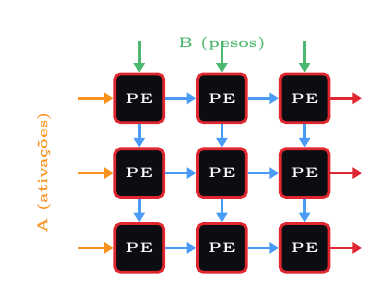
\begin{tikzpicture}[x=1cm,y=1cm, pe/.style={draw=vermelho, line width=1pt, rounded corners=2pt, fill=fundo, minimum size=0.62cm, font=\tiny\bfseries, text=titulo},
  ar/.style={-{Triangle[length=1.2mm,width=1.4mm]}, line width=1pt}]
  \foreach \r in {0,1,2}{\foreach \c in {0,1,2}{\node[pe] (p\r\c) at (\c*1.05,-\r*0.95) {PE};}}
  \foreach \r in {0,1,2}{\draw[ar,laranja] ($(p\r0.west)+(-0.45,0)$) -- (p\r0.west);
    \draw[ar,azul] (p\r0.east) -- (p\r1.west); \draw[ar,azul] (p\r1.east) -- (p\r2.west);
    \draw[ar,vermelho] (p\r2.east) -- ++(0.4,0);}
  \foreach \c in {0,1,2}{\draw[ar,verde] ($(p0\c.north)+(0,0.4)$) -- (p0\c.north);
    \draw[ar,azul] (p0\c.south) -- (p1\c.north); \draw[ar,azul] (p1\c.south) -- (p2\c.north);}
  \node[font=\tiny\bfseries, text=verde, anchor=south] at (1.05,0.48) {B (pesos)};
  \node[font=\tiny\bfseries, text=laranja, rotate=90, anchor=south] at (-1.0,-0.95) {A (ativações)};
\end{tikzpicture}
\end{minipage}
\tradeoff{arrays maiores processam mais dados por ciclo, mas custam área e potência. A quantização Int8 reduz memória,
banda e energia por operação, aceitando perda de precisão.}
\end{conceito}

\begin{faca}
\begin{passos}
  \item Abra a aba \gui{NPU}: \gui{INPUT MEMORY (A)} traz valores de 1 a 9 e \gui{WEIGHT MEMORY (B)}, a matriz identidade.
        Antes de rodar, preveja o resultado de $C = A \times B$.
  \item Clique uma vez em \btn{Step Clock}: \gui{Global Clock} vai de 0 para 1 e \cod{A[0][0]} e \cod{B[0][0]} ficam destacadas,
        entrando no \cod{PE\_00}.
  \item Continue clicando, acompanhando \cod{a*b} e o acumulador dentro de cada PE. Anote em que ciclo cada PE mostra
        \gui{DONE} e, ao final (8 ciclos), compare \gui{OUTPUT MEMORY (C)} com a sua previsão.
  \item Reinicie a simulação, edite \cod{A[0][0]} para $-20$ e ative \gui{Add Bias (+5)} no \gui{PPU PIPELINE}
        (o \gui{ReLU Activation} já vem ligado). Rode com \btn{Auto Run}.
  \item Edite \cod{A[2][2]} para 600, ative \gui{Quantization (Int8)} e rode de novo, observando os valores de saída.
\end{passos}
\end{faca}

\begin{discuta}
  \item Em que ordem os PEs mostraram \gui{DONE}?
        \esperado{Em diagonais: PEs com o mesmo $r+c$ terminam juntos e cada diagonal termina um ciclo depois da anterior; o \texttt{PE\_22} é o último, pois os dados atravessam a grade um PE por ciclo.}
  \item Quanto passou a valer \cod{C[0][0]} com $A[0][0] = -20$, bias e ReLU? E \cod{C[2][2]} com 600 e Int8?
        \esperado{Multiplicar pela identidade preserva a matriz. $-20+5 = -15 \rightarrow$ ReLU $\rightarrow 0$. $600+5 = 605 \rightarrow 605 \gg 2 = 151 \rightarrow$ saturado em 127.}
  \item Um acumulador vale $-6$ antes da PPU. Qual a saída com Bias $\rightarrow$ ReLU? E se a ordem fosse ReLU $\rightarrow$ Bias?
        Por que a ordem não pode ser escolhida à vontade?
        \esperado{$-6 \rightarrow -1 \rightarrow 0$, contra $-6 \rightarrow 0 \rightarrow 5$ na ordem invertida. O hardware precisa repetir a ordem usada no treinamento da rede, senão a inferência muda.}
  \item Com a quantização ativa, quanto vira um acumulador igual a 3? O que isso revela sobre usar sempre o mesmo fator de escala?
        \esperado{$3 \gg 2 = 0$: a informação se perde mesmo cabendo em 8 bits. Por isso redes reais calibram a escala por camada antes de quantizar.}
\end{discuta}
\borda{arranjos sistólicos estão na base de aceleradores como a TPU do Google. Na FPGA desta plataforma, a NPU chega a ser
até 5000$\times$ mais rápida que a execução escalar na CPU.}

% ------------------------------ 06 -------------------------------------
\estacao{ambar}{06}{Tiling: Escalando o Hardware}{Tiling}{Simulação}{5 min}
\begin{conceito}
O array do experimento 5 tem tamanho fixo, definido na fabricação, mas redes reais usam matrizes muito maiores. O
\textbf{tiling} resolve isso por controle (multiplexação no tempo), não por hardware: as matrizes são divididas em blocos do tamanho do array, que é
reutilizado várias vezes. Para 6$\times$6 com um array 3$\times$3, cada quadrante de $C$ soma \textbf{duas} multiplicações de blocos:
\[
\begin{bmatrix} A_{11} & A_{12}\\ A_{21} & A_{22}\end{bmatrix}
\times
\begin{bmatrix} B_{11} & B_{12}\\ B_{21} & B_{22}\end{bmatrix}
=
\begin{bmatrix}
{\color{laranja}A_{11}B_{11}} + {\color{azul}A_{12}B_{21}} & {\color{laranja}A_{11}B_{12}} + {\color{azul}A_{12}B_{22}}\\[1mm]
{\color{laranja}A_{21}B_{11}} + {\color{azul}A_{22}B_{21}} & {\color{laranja}A_{21}B_{12}} + {\color{azul}A_{22}B_{22}}
\end{bmatrix}
\]
A primeira parcela ({\color{laranja}\textbf{P1}}) escreve o quadrante; a segunda ({\color{azul}\textbf{P2}}) acumula e o finaliza.
\tradeoff{tempo vs.\ área. Um array 6$\times$6 faria tudo em um passe, mas com 36 PEs em vez de 9; o tiling reaproveita o
array menor à custa de mais passos e de movimentação de dados, que costuma gastar mais energia que a própria conta.}
\end{conceito}

\begin{faca}
\begin{passos}
  \item Abra a aba \gui{Tiling}. As matrizes \gui{MATRIX A (INPUT)}, \gui{MATRIX B (WEIGHTS)} e
        \gui{MATRIX C (OUTPUT)} são divididas em quatro quadrantes de $3\times3$. As matrizes A e B
        contêm os dados de entrada, enquanto C começa zerada. Observe que, embora o resultado seja uma
        matriz $6\times6$, a NPU possui apenas uma unidade de processamento $3\times3$.

  \item Clique em \btn{Step Tile}. Observe os quadrantes de A e B carregados na NPU e o quadrante
        correspondente de C. O \gui{NPU Core} indica \cod{LOADING TILES... MULTIPLY}, representando
        a primeira operação parcial (\gui{P1}) necessária para calcular aquele quadrante do resultado.

  \item Consulte o \gui{TILING STATE MACHINE LOG} e identifique a operação realizada. Por exemplo,
        \cod{C\_11 (P1) = A\_11 * B\_11} indica que os primeiros tiles de A e B são multiplicados
        para produzir a primeira parcela de $C_{11}$.

  \item Clique novamente em \btn{Step Tile}. Observe que o mesmo quadrante de C é calculado novamente,
        mas agora no modo \cod{MULTIPLY + ACCUMULATE}. A segunda parcela é somada à primeira, como em
        \cod{C\_11 (P2) = C\_11 + (A\_12 * B\_21)}. Quando o cálculo é concluído, o log indica
        \cod{[C\_11 DONE]} e o quadrante é escrito na memória.

  \item Continue avançando com \btn{Step Tile} até completar os oito passos. Observe que
        cada quadrante $3\times3$ de C é obtido pela soma de duas multiplicações de tiles $3\times3$.

  \item Clique em \btn{Reset Data} para restaurar os dados iniciais e, em seguida, em \btn{Auto Run}.
        Acompanhe a execução automática, com um passo a cada 1,2 s, até que todos os oito passos sejam
        concluídos e seja exibida a mensagem
        \cod{[SUCESSO] Multiplicação 6x6 concluída usando hardware 3x3!}.
\end{passos}
\end{faca}

\begin{discuta}
  \item Quantos passos foram necessários e por que não 4? Em que ordem os quadrantes de $C$ foram concluídos?
        \esperado{8: são 4 quadrantes e cada um precisa de P1 e P2. A ordem foi $C_{11}, C_{11}, C_{12}, C_{12}, C_{21}, C_{21}, C_{22}, C_{22}$: cada quadrante termina antes de o próximo começar.}
  \item Quais blocos de A e B formam $C_{12}$ e $C_{21}$? Confira com o log.
        \esperado{$C_{12} = A_{11}B_{12}$ (P1) $+ A_{12}B_{22}$ (P2) e $C_{21} = A_{21}B_{11}$ (P1) $+ A_{22}B_{21}$ (P2).}
  \item Se cada passo roda o array 3$\times$3 por 8 ciclos, quanto custa a multiplicação 6$\times$6? Quantos passos exigiriam uma
        matriz 9$\times$9 e uma 7$\times$7, que precisa de \emph{zero-padding}? Que desperdício o padding introduz?
        \esperado{$8 \times 8 = 64$ ciclos. Passos $= (K/N)^3$: 9$\times$9 dá 27, e a 7$\times$7 é completada até 9$\times$9, também com 27. Os PEs gastam ciclos e energia com MACs do tipo $0 \times$ valor.}
\end{discuta}
\borda{bibliotecas como cuDNN e oneDNN usam tiling para rodar matrizes enormes em hardware fixo. Nos resultados do TCC, a NPU
gasta os mesmos 25.264 ciclos com matriz densa ou 80\% esparsa: o array não pula zeros.}

% ------------------------------ 07 -------------------------------------
\estacao{magenta}{07}{Inferência MNIST em FPGA}{Neural Network}{FPGA}{7 min}
\begin{conceito}
Uma rede neural tem duas fases. No \textbf{treinamento}, os parâmetros são ajustados com milhares de exemplos, em um
computador com recursos: aqui, PyTorch no próprio PC. Na \textbf{inferência}, os pesos ficam congelados e cada entrada
nova gera uma predição, e é essa fase que precisa rodar na borda. Os pesos de uma camada convolucional e de uma totalmente
conectada são enviados à NPU pela serial. Cada desenho é recortado, redimensionado para 20$\times$20 e centralizado em
28$\times$28, como no dataset MNIST, e então quantizado em Int8 e enviado byte a byte. A NPU devolve 10 \emph{logits} e a
GUI mostra $\mathrm{softmax}(\text{logits}/T)$, com $T = 15$.
\par\medskip
\centering
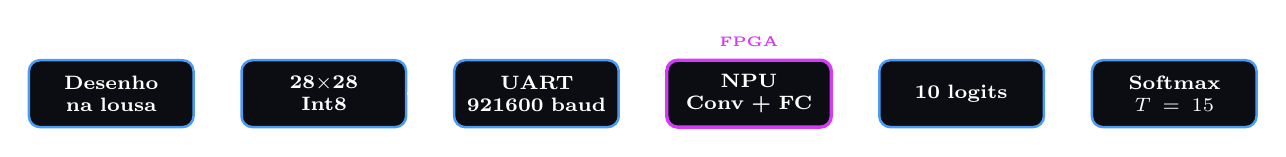
\begin{tikzpicture}[x=1cm,y=1cm, font=\scriptsize,
    pc/.style={draw=azul, line width=0.9pt, rounded corners=4pt, fill=fundo, text=titulo, minimum height=0.85cm, text width=1.95cm, align=center, inner sep=2pt},
    hw/.style={draw=magenta, line width=1.2pt, rounded corners=4pt, fill=fundo, text=titulo, minimum height=0.85cm, text width=1.95cm, align=center, inner sep=2pt},
    ar/.style={-{Triangle[length=1.4mm,width=1.6mm]}, line width=0.9pt, titulo}]
  \node[pc] (n1) at (0,0) {\bfseries Desenho\\na lousa};
  \node[pc] (n2) at (2.7,0) {\bfseries 28$\times$28\\Int8};
  \node[pc] (n3) at (5.4,0) {\bfseries UART\\921600 baud};
  \node[hw] (n4) at (8.1,0) {\bfseries NPU\\Conv + FC};
  \node[pc] (n5) at (10.8,0) {\bfseries 10 logits};
  \node[pc] (n6) at (13.5,0) {\bfseries Softmax\\$T = 15$};
  \foreach \a/\b in {n1/n2,n2/n3,n3/n4,n4/n5,n5/n6}{\draw[ar] (\a) -- (\b);}
  \node[font=\tiny\bfseries, text=magenta, anchor=south] at ($(n4.north)+(0,0.03)$) {FPGA};
\end{tikzpicture}
\par\raggedright
\tradeoff{modelos maiores tendem a ser mais precisos, mas também mais lentos e caros em área. Treinar no PC e inferir
na FPGA evita tanto o custo de treinar na borda quanto a latência de depender da nuvem.}
\end{conceito}

\begin{faca}
\begin{passos}
  \item Abra a aba \gui{Neural Network Inference (MNIST)}. A lousa começa bloqueada, pois ainda não há pesos na NPU.
  \item Clique em \btn{Programar FPGA}. Acompanhe as mensagens:
        calibração do modelo, conexão serial, upload do firmware e transferência dos pesos Conv2D via DMA.
  \item Aguarde ``FPGA Programada com Sucesso!'' e o indicador \gui{NPU Core} em \gui{IDLE / READY}.
  \item Desenhe um dígito em \gui{ENTRADA DE DESENHO (0-9)}. Observe a
        \gui{VISÃO DA NPU (28x28)}: é a imagem exata enviada ao hardware.
  \item Solte o mouse e leia o dígito em \gui{PREVISÃO}, a \gui{LATÊNCIA} e as dez barras de \gui{CONFIANÇA}.
  \item Clique em \btn{LIMPAR LOUSA} e repita com um ``7'' que lembre um ``1'' e, depois, com um ``X''.
\end{passos}
\end{faca}

\begin{discuta}
  \item Como a distribuição de confiança mudou entre o dígito bem desenhado e o ambíguo?
        \esperado{No dígito claro, uma barra perto de 100\%. No ambíguo, a barra vencedora cai e aparece uma concorrente (1 ou 7) com porcentagem relevante: incerteza real na entrada vira incerteza na saída.}
  \item A rede se recusou a classificar o ``X''? Que limitação isso revela, e como ela poderia ser mitigada?
        \esperado{Não: o softmax sempre distribui 100\% entre as 10 classes, então a rede escolhe a opção menos ruim. Mitigações: limiar mínimo de confiança, classe extra de rejeição ou detecção de entradas fora da distribuição.}
  \item A rede utiliza dados no formato \cod{INT8}, enquanto o processador é RV32I e possui registradores de 32 bits.
        Como esses dois fatos se relacionam? O que acontece quando um valor \cod{INT8} é manipulado por uma instrução
        como \cod{mv}?
        \esperado{O RV32I trabalha com registradores de 32 bits, enquanto os pesos e ativações da rede podem ser
        representados com apenas 8 bits. A instrução \cod{mv} é uma pseudoinstrução para \cod{addi rd, rs1, 0} e
        movimenta o conteúdo de um registrador de 32 bits; ela não realiza uma conversão automática para \cod{INT8}.
        Portanto, um valor INT8 precisa ser armazenado ou empacotado dentro de um registrador de 32 bits, considerando
        extensão de sinal, zero extension e/ou operações de \textit{packing} e \textit{unpacking}, conforme a aplicação.
        Essa diferença de largura mostra por que aceleradores de Edge AI podem explorar operações de baixa precisão,
        como INT8, para realizar mais operações por ciclo e reduzir o tráfego de memória em comparação com dados de
        maior precisão.}
\end{discuta}
\borda{palavras de ativação em assistentes de voz e câmeras inteligentes fazem inferência local por latência, privacidade e
energia. Aqui, todos os experimentos anteriores trabalham juntos.}

% ------------------------------ FECHAMENTO ------------------------------
\clearpage
\colorlet{acc}{verde}
\secao{Fechamento: da sala de aula à Edge AI}
{\small Resumo para consulta: o que cada experimento mostrou e onde isso aparece em um sistema de computação na borda.}
\par\vspace{4mm}
{\small\arrayrulecolor{borda}\renewcommand{\arraystretch}{1.45}
\noindent\begin{tabularx}{\linewidth}{|>{\centering\arraybackslash}m{0.7cm}|>{\raggedright\arraybackslash}m{4.9cm}|>{\raggedright\arraybackslash}X|}
\hline
\rowcolor{painelB}{\footnotesize\bfseries\color{titulo}\#} & {\footnotesize\bfseries\color{titulo}Conceito clássico} & {\footnotesize\bfseries\color{titulo}No sistema de borda} \\ \hline
{\bfseries\color{laranja}1} & Datapath multiciclo e FSM & Núcleo simples que orquestra um SoC heterogêneo \\ \hline
{\bfseries\color{verde}2}   & E/S mapeada em memória & Firmware bare-metal controlando periféricos e a NPU \\ \hline
{\bfseries\color{vermelho}3}& Barramento e arbitragem & Dados movidos sem a CPU; o barramento vira gargalo \\ \hline
{\bfseries\color{azul}4}    & Interrupções & RTOS preemptivo reagindo a eventos com baixo consumo \\ \hline
{\bfseries\color{roxo}5}    & ULA e multiplicação & Acelerador MAC paralelo com quantização Int8 \\ \hline
{\bfseries\color{ambar}6}   & Localidade e hierarquia de memória & Hardware de tamanho fixo reutilizado por blocos \\ \hline
{\bfseries\color{magenta}7} & Sistema completo & Inferência local: latência, privacidade e energia \\ \hline
\end{tabularx}}

\vspace{10mm}
\colorlet{acc}{vermelho}
\begin{tarefabox}{TAREFA FINAL \textperiodcentered\ ENTREGA DO DOCUMENTO EM GRUPO}
Ao final da aula, cada grupo entrega um documento com:
\begin{itemize}
  \item a identificação do grupo (nomes e RAs);
  \item as respostas das perguntas de \textbf{Observe e discuta em grupo} dos sete experimentos, numeradas como no roteiro
        (1.1, 1.2, \dots, 7.4);
  \item os valores observados na GUI que sustentam cada resposta, como contagens de ciclos, Total Clocks, CPU Stalls e latências.
\end{itemize}
\vspace{1mm}
\ifgabarito
\par\vspace{2mm}{\footnotesize\color{gab}\textbf{Professor:} as respostas esperadas estão logo abaixo de cada pergunta, nas páginas dos experimentos.}
\fi
\end{tarefabox}

\end{document}